%begin-include

% What I want to talk about in this section?
% - Cells signaling pathways are part of the cell communication system,
% and it allows the cell to perceive the conditions of the environment 
% and also to change its behaviour according to the input signal.
% - The signals perceived by a cell can come from cells that very close
% (including itself), as in synapses or it can travel long distances in 
% the organism, as in hormones.
% - When a signal reaches a cell, it can either activate a receptor in
% the cell membrane or diffuse into the cell.
% - Once this happen, the signal or the activated receptor can trigger
% a sequence of chemical interaction, altering the conformation and 
% state of proteins and also changing the concentration of chemical 
% species in the cell. Ultimately, this chain of effects can alter the 
% behaviour of the cell, what is called signal transduction.
% - Studying signaling pathways is important because they help us 
% understand the mechanisms of a cell, which can for example, elucidate 
% treatments for diseases.
\section{Cell Signaling Pathways}
Cell signaling pathways are part of the complex cell communication 
system, and it allows the cell to perceive the conditions of the 
environment in which it is placed and change its behaviour accordingly.
Signaling pathways participate in the regulation of many cell functions,
including development, division and cell death. Bad functioning 
signaling pathways can also be related to diseases, as in many cases of
cancer.

The signal perceived by a cell can come from cells that are close 
(including the same cell that produced the signal), as in synapses, or 
it can travel long distances in the organism, as in hormones. When a 
signal reaches a cell, it can either penetrate the cell or bind to some 
specific receptor in the membrane. Once either of those events happen, 
the signal or the receptor can trigger a sequence of chemical 
interactions that can include change of conformation of proteins, 
activation or inactivation of proteins, and change of concentration of
chemical species in the cell. Ultimately, this chain of chemical 
reactions caused by the signal can alter the behaviour of the cell, what 
is called signal transduction.

Since signaling pathways participate in many of the cell functions, and 
are also related to diseases, it is important to study those structures
in order to get a better understanding of the cell mechanisms and 
diseases. One approach on the study of the cell signaling pathways is to 
measure the concentration change of proteins that participate on the 
pathway of interest.

% - Western blot is a technique that can indicate the amount of a 
% specific protein that is in a mixture of proteins
% - This technique shows the presence of a protein in a mixture by 
% ``blotting'' these molecules into a membrane. 
% - Repeating the procedure in different times define time-course 
% observations of the protein in a biological experiment.
% - With these observations in hand, the researcher is able to construct 
% a measurement that is relevant to describe the biological experiment. 
% For instance, in a signaling network where a protein is closely 
% related to the behaviour of interest of the cell, this protein is a 
% good candidate as a measure of the system.
\section{Measurements of Proteins in Cell Signaling Pathways}
Western blot is a laboratory technique that can indicate the amount of a
specific protein that is present in a mixture. This technique show the 
presence of a protein in a mixture by ``blotting'' a membrane where the 
molecules of interest are located. We can superficially summarize the 
procedure in the following steps: first a mixture containing a sample of 
cells of interest must be created; second, proteins from the mixture 
should be fixed on the blotting membrane; third, an antibody should bind 
to the target protein molecules; and finally, a method for highlighting 
the bound antibody should be applied. An image of the resulting membrane 
can then be analyzed with computer programs to quantify the relative 
concentration (with respect to some other protein, usually a control 
protein that has fairly the same concentration during the whole 
experiment) of the protein of interest.

By repeating this procedure in different times it is possible to create 
time-course observations of proteins throughout the biological 
experiment. With this tool, a researcher can choose a set of relevant 
proteins from a signaling network and gain knowledge about the dynamics 
of such chemical species during the experiment. For instance, in a 
signaling network experiment in which it is desired to understand how
the change of concentrations of a species at the beginning of the 
pathway changes the concentration of some species at the end of the 
cascade, then measurements of both are relevant to understand the 
biological experiment. Figure~\ref{fig:western_blot_example} presents an 
example of time-course Western blot for an experiment where it is 
desirable to understand how extracellular signal-regulated kinase (ERK)
is activated (phosphorylated) as a function of levels of Rat sarcoma
bound to guanosine triphosphate (Ras-GTP).

\begin{figure}[!ht]
\centering
    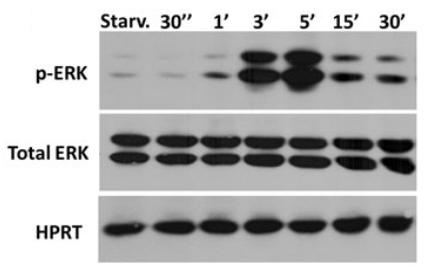
\includegraphics[width=\textwidth]{fundamental_concepts/western_blot.png}
    \caption{Figure {\bf a} shows time-course measurements of ERK, 
    phosphorylated ERK and hypoxanthine-guanine 
    phosphoribosyltransferase (HPRT). HPRT is a ``loading'' protein, 
    that means that its concentration is fairly the same through the 
    experiment, and therefore it is used as a normalizing factor to 
    total ERK concentration. Figure  {\bf b} shows values of 
    phosphorylated ERK that are obtained after processing figure 
    {\bf a}. Original image of Marcelo S. Reis et al. 
    (2017)~\cite{Reis2017}.}
    \label{fig:western_blot_example}
\end{figure}

These measurements alone do not always provide means for researchers to 
understand a cell signaling pathway experiment. However, if we create a 
computational models for this signaling networks that is able to 
reproduce experimental data, then it is possible to use this model as a 
summary of the signaling network, which can provide to researchers 
evidences of the biological phenomena.


% What do I need to talk about?
% - We can model the concentration changes of chemical species as 
% differential equations, using the mass-action kinetic laws
% - The mass action kinetic law states that in an elementary reaction,
% the rate of a chemical reaction is directly proportional to the 
% product of the reactants concentrations.
% - What is elementary?
% 2.1 Elementary reactions rate equations
% - Types of elementary: first order reaction and second order reaction
% - How do we write up these two? 
% - Chemical notation with constants
% - From there we can write a system of differential equations to 
% describe the signaling pathway.
% - As an example, let's show the equations for a simple enzymatic 
% equation.
% 2.2 Simplifications of reactions
% - More can be done. We can simplify some equations 
% 2.1 Mass conservation simplification
% 2.2
\section{Dynamic Modeling of Cell Signaling Pathways}
One approach onto modeling cell signaling pathways is to model the 
dynamics of the concentrations of chemical species involved. This can be
accomplished when using the law of mass action. This law states that, 
in an elementary reaction, the speed (or rate) of a chemical reaction is 
proportional to the product of the concentration of all reactants. An 
elementary reaction is a reaction in which there is no participation or 
need of an intermediate reaction to describe the first in a molecular 
level. In practice, it is more common to see two types of elementary 
reactions, they are first or second order reactions. 

\subsection{Modeling Elementary Reaction Rates}
A first order reaction is composed of one reactant only. Suppose A is 
the only reactant and B is the only product of a reaction, then we can
write this reaction as:
\begin{equation*}
\ce{
    A -> B
}
\end{equation*}
The reaction rate of this reaction, according to the law of mass 
action, is 
\begin{equation*}
    k_1[\text{A}]
\end{equation*}
where $k_1$ is some constant and [A] is the concentration of A. 

A second order reaction is composed of two reactants. Suppose C and D 
are both and the only reactants and F is the product of a reaction, then
we can write this reaction as:
\begin{equation*}
\ce{
    C + D -> F
}
\end{equation*}
The reaction rate of this reaction is:
\begin{equation*}
    k_2\text{[C][D]}
\end{equation*}
where $k_2$ is a constant and [C] and [D] are the concentrations of C 
and D, respectively.

Using these two laws to calculate the speed of reactions, we are able 
to describe how the concentration of chemical species in a system change 
though time using differential equations. To illustrate this and future 
concepts of this section, we are going to consider a minimal system 
composed of a simple enzymatic reaction:
\begin{equation}
\ce{
    E + S <=>[\ce{$k$_f}][\ce{$k$_r}] ES ->[\ce{$k_{cat}$}] E + P
}
\label{eq:simple_enzymatic}
\end{equation}
where E is an enzyme, S is the substrate, ES is the enzyme-substrate
complex, and P is a product

Each arrow in equation~\ref{eq:simple_enzymatic} represents one 
elementary reaction, and the names over or under arrows represent 
reaction rate constants. All three reactions can be represented by the
equations:

%The first reaction has E and S as reactants and
%ES as a product, and can be written as 
\begin{equation}
\ce{
    E + S ->[\ce{$k_f$}] ES 
}
\label{eq:es_complex_fwd}
\end{equation}
%and has reaction rate of $k_f$[E][S]. Second, the reverse of the first 
%reaction has ES as reactant and both E and S as product,
\begin{equation}
\ce{
    ES ->[$k_r$] E + S
}
\label{eq:es_complex_rev}
\end{equation}
%and has reaction rate 
\begin{equation}
\ce{
    ES ->[$k_{cat}$] E + P
}
\label{eq:es_pe}
\end{equation}
and they have, respectively, reaction rates of:
\begin{equation*}
\begin{aligned}
    & k_f\text{[E][S]} \\
    & k_r\text{[ES]} \\
    & k_{cat}\text{[ES]}
\end{aligned}
\end{equation*}

{\color{blue} TODO: Maybe I should stop this subsection here and start another
where I explain what comes next as "Dynamic Modeling of a System of Reactions"}

Now, to determine a model of the concentration dynamics of every 
chemical species involved in reaction~\ref{eq:simple_enzymatic}, we will
write a system of ordinary differential equations. To do so, for every 
species we should calculate the rate of its change based on the rate of 
each reaction that it participates. For instance, the enzyme E is a 
reactant on reaction~\ref{eq:es_complex_fwd} and is also a product on 
reactions~\ref{eq:es_complex_rev} and~\ref{eq:es_pe}, then we consider 
that E changes its concentration over time ($t$) according to the 
differential equation:
\begin{equation}
    \frac{d[\text{E}]}{dt} = -k_f\text{[E][S]} + (k_r + k_{cat}) \text{[ES]}
\end{equation} 
Repeating this procedure for every other species of the enzymatic 
reaction induces the desired system of ordinary differential equations:
\begin{equation}
    \begin{aligned}
        \frac{d[\text{E}]}{dt} = & -k_f\text{[E][S]} + (k_r + k_{cat}) \text{[ES]} \\
        \frac{d[\text{S}]}{dt} = & -k_f\text{[E][S]} + k_r\text{[ES]} \\
        \frac{d[\text{ES}]}{dt} = & k_f\text{[E][S]} - (k_r + k_{cat}) \text{[ES]} \\
        \frac{d[\text{P}]}{dt} = &  k_{cat}\text{[ES]} \\
    \end{aligned}
\end{equation}

\subsection{Simplifications of Dynamic Models}

\section{Identification of Cell Signaling Pathways}
\section{State of the Art in Model Selection}
%\section{Bayesian Inference}
%\subsection{Girolami (bioinformatics)}
%\subsection{Kolch}
%\subsection{ABC-Sysbio}
